\documentclass[aspectratio=169,11pt]{beamer}

\usetheme{Madrid}
\usecolortheme{default}
\usefonttheme{professionalfonts}
\setbeamertemplate{navigation symbols}{}
\setbeamertemplate{footline}[frame number]

\usepackage{amsmath, amssymb, booktabs, graphicx}
\graphicspath{{../../assets/figures/}{assets/figures/}}

\title{Labor Demand and Production}
\subtitle{Labor II --- Week 1}
\author{Teaching deck draft}
\date{}

\begin{document}

\begin{frame}
  \titlepage
\end{frame}

\begin{frame}{Central question}
\begin{itemize}
    \item How do firms choose labor input in a static production setting?
    \item Which objects belong to substitution across inputs, and which belong to scale?
    \item Why do labor-demand elasticities matter for policy incidence and for the rest of Labor II?
\end{itemize}
\end{frame}

\begin{frame}{Course reorientation}
\begin{itemize}
    \item Labor I centered workers, households, and worker-side policy.
    \item Labor II begins inside the firm: employment is now an input-demand object.
    \item Week 1 is deliberately static: no adjustment costs yet, no bargaining yet, no monopsony yet.
\end{itemize}
\end{frame}

\begin{frame}{Labor I to Labor II bridge}
\begin{itemize}
    \item Labor I asked how workers respond to wages, taxes, and institutions.
    \item Week 1 asks where firms want to be after those same wedges change.
    \item Week 2 will ask why firms often do not get there immediately.
\end{itemize}
\end{frame}

\begin{frame}{Production and the static firm problem}
\[
q = F(L,K;A)
\qquad
pF_L(L,K;A)=w
\]

\begin{itemize}
    \item Labor demand is derived from technology, product demand, and factor prices.
    \item The value of the marginal product benchmark is useful but not enough.
    \item We need cost minimization to separate substitution from scale.
\end{itemize}
\end{frame}

\begin{frame}{Cost minimization and conditional labor demand}
\[
\min_{L,K} \; wL+rK
\quad \text{s.t.} \quad
F(L,K;A)\ge q
\]
\[
\frac{F_L}{F_K} = \frac{w}{r}
\qquad
\eta^{c}_{LL}=-(1-s_L)\sigma
\]

\begin{itemize}
    \item Conditional demand holds output fixed.
    \item It isolates substitution across inputs.
    \item It is not yet the full observed employment response to a labor-cost shock.
\end{itemize}
\end{frame}

\begin{frame}{Isoquant and isocost geometry}
\begin{center}
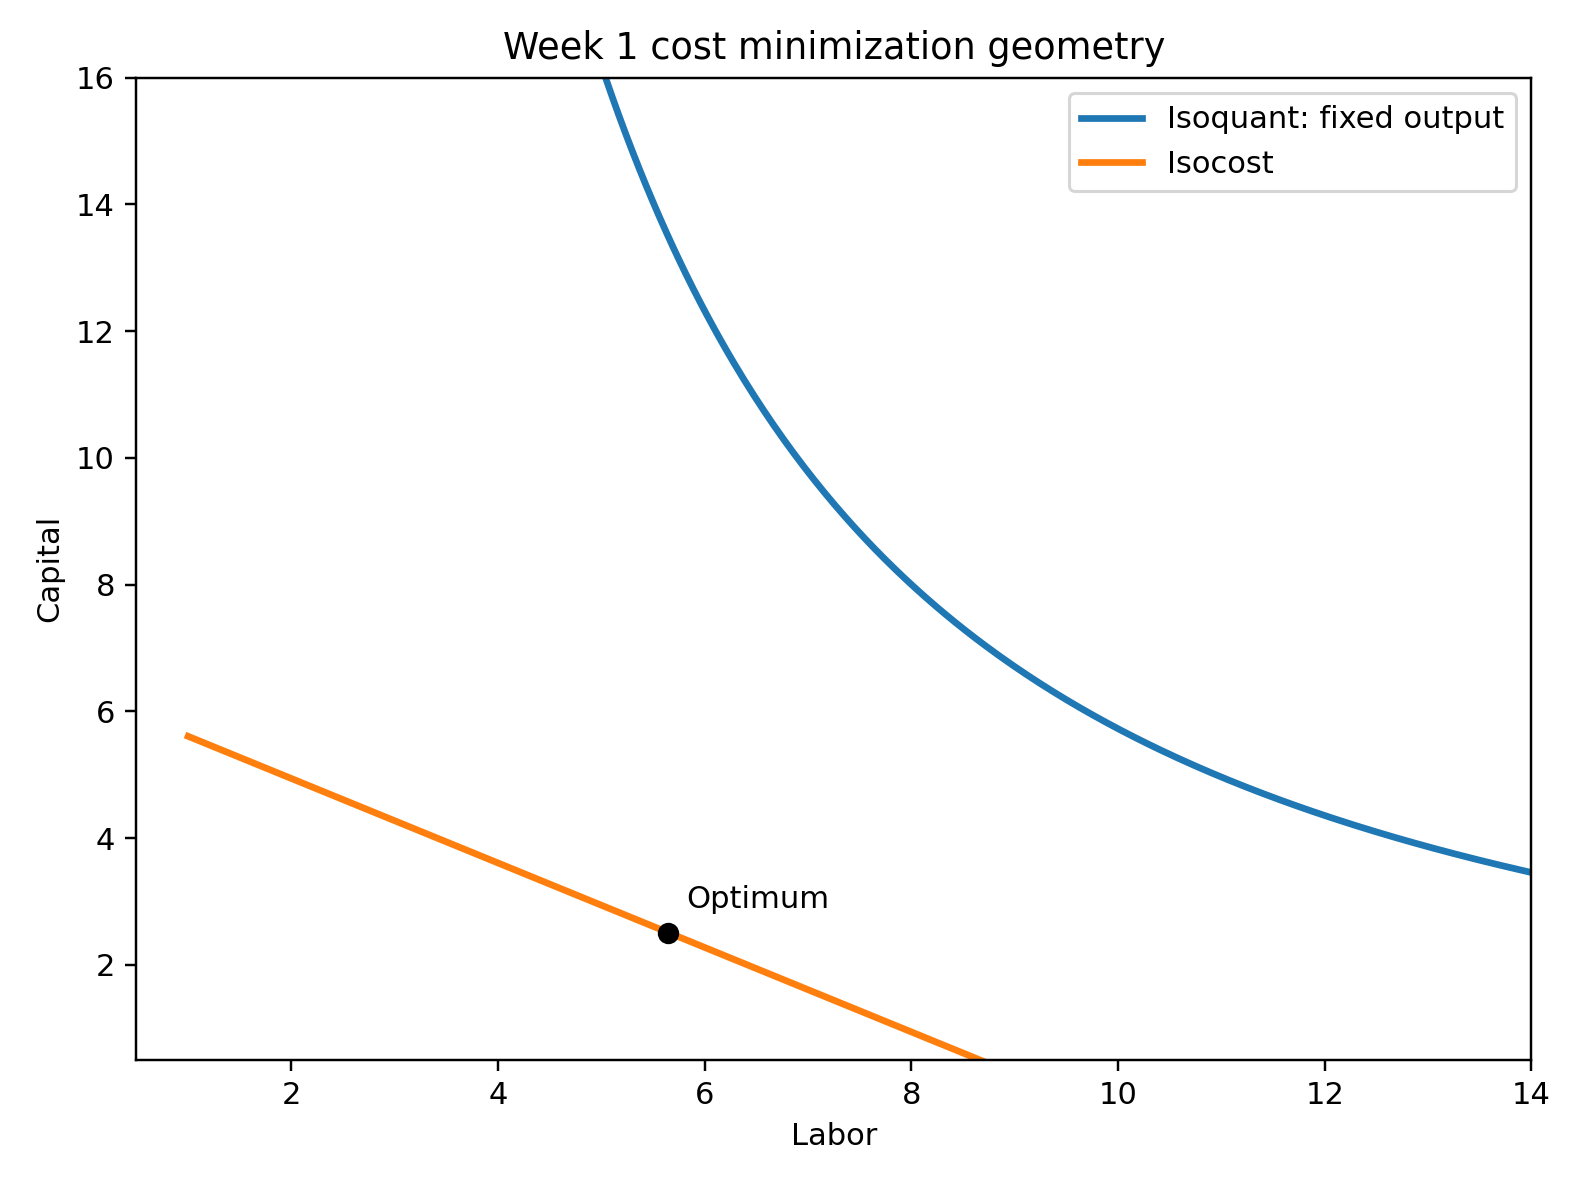
\includegraphics[width=0.83\linewidth]{01-static-labor-demand-isoquant-isocost.png}
\end{center}
\end{frame}

\begin{frame}{Unconditional labor demand and scale effects}
\[
\frac{d\ln L}{d\ln w}
=
\underbrace{\frac{\partial \ln L^{c}}{\partial \ln w}\Big|_{q}}_{\text{substitution}}
+
\underbrace{\frac{\partial \ln L}{\partial \ln q}\frac{d\ln q}{d\ln w}}_{\text{scale}}
\]
\[
\eta_{LL}=-(1-s_L)\sigma-s_L\eta
\]

\begin{itemize}
    \item Total labor demand combines input substitution with output contraction.
    \item Product-demand elasticity matters because cost shocks change desired scale.
\end{itemize}
\end{frame}

\begin{frame}{Conditional versus total demand}
\begin{center}
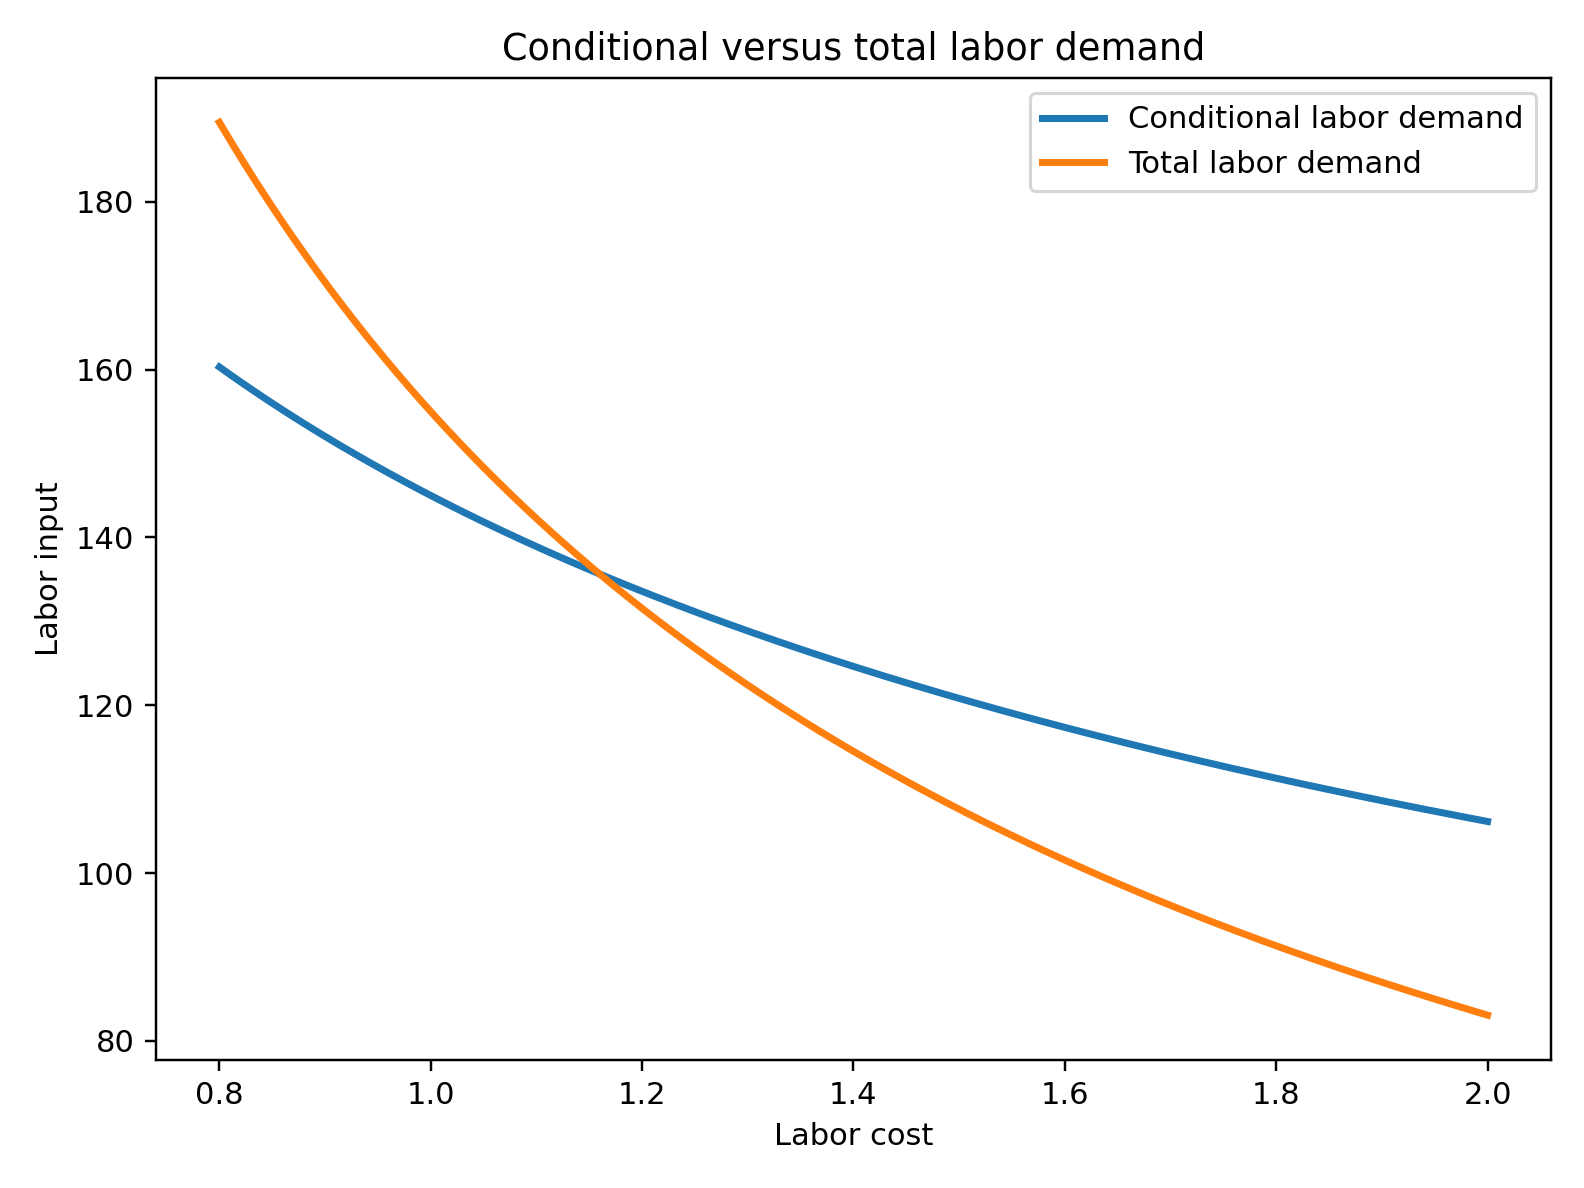
\includegraphics[width=0.85\linewidth]{01-conditional-vs-unconditional-demand.png}
\end{center}
\end{frame}

\begin{frame}{Hicks--Marshall laws}
\begin{itemize}
    \item Labor demand is more elastic when substitution away from labor is easier.
    \item Labor demand is more elastic when product demand is more elastic.
    \item Labor demand is more elastic when labor is a larger share of cost.
    \item Labor demand is more elastic when other inputs are easier to expand.
\end{itemize}

\begin{center}
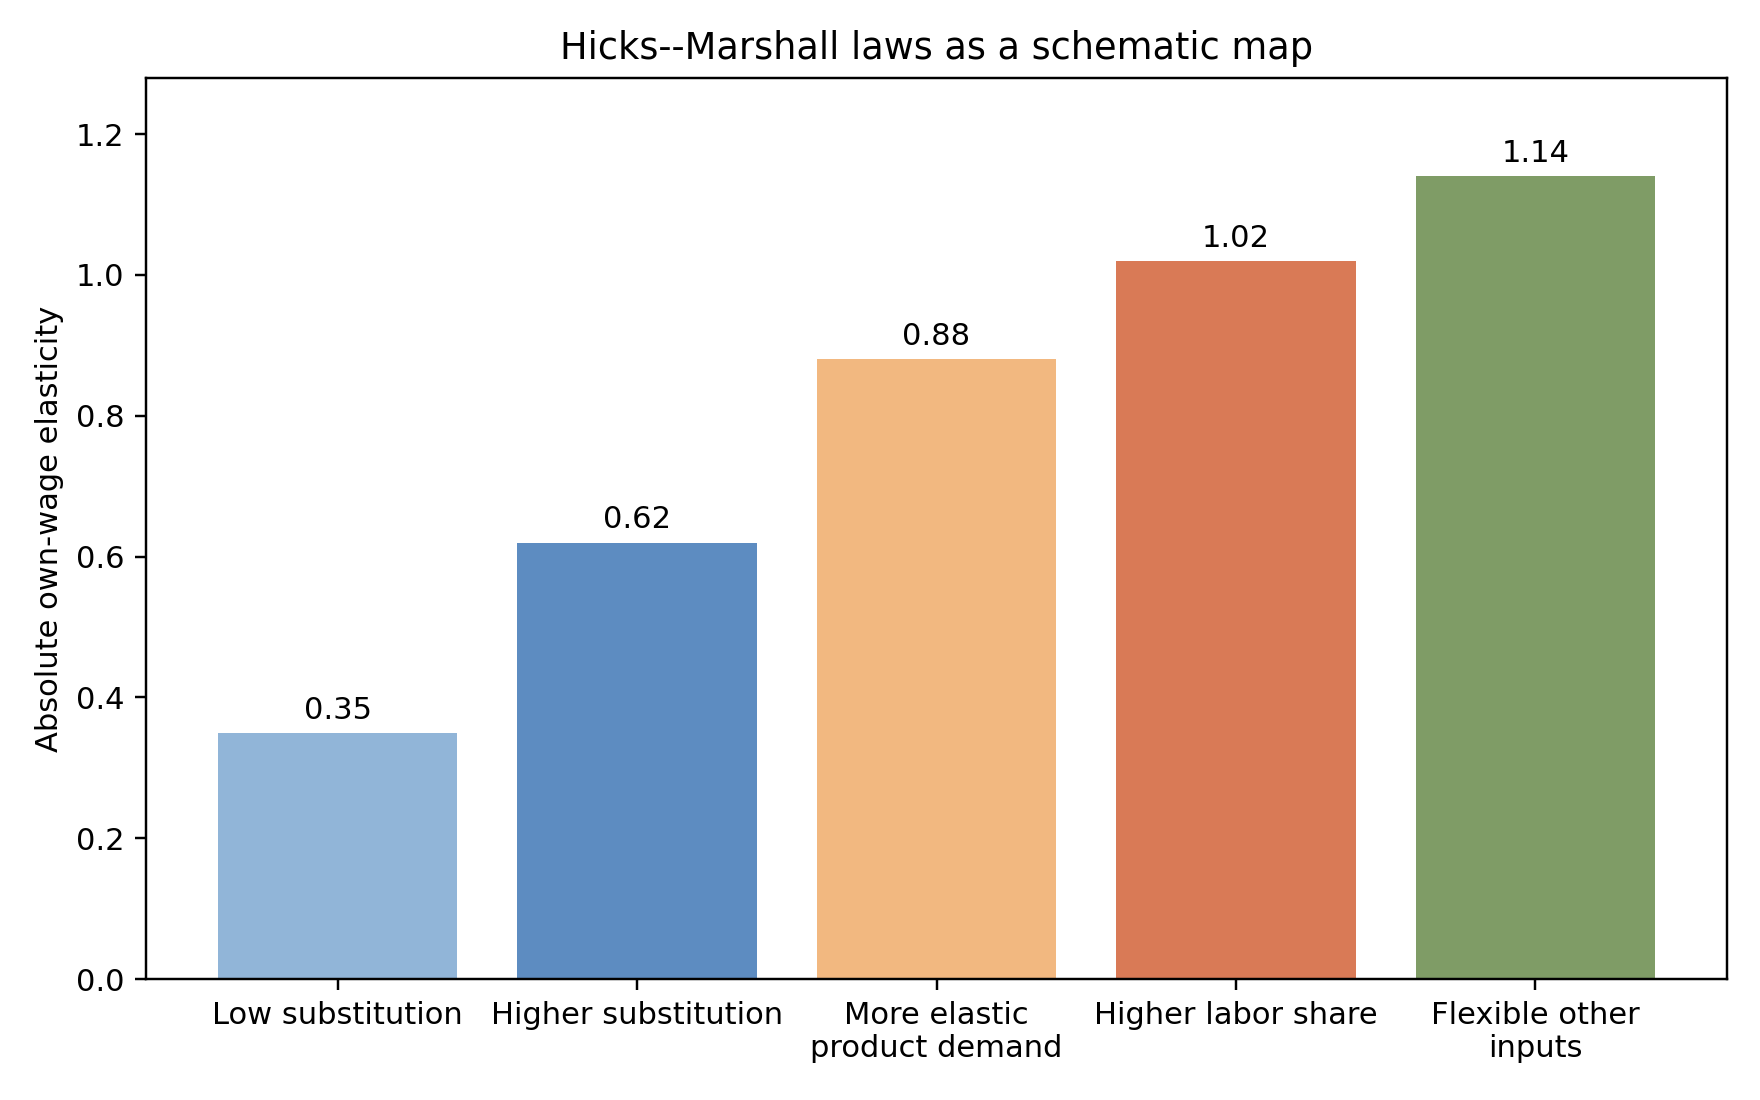
\includegraphics[width=0.62\linewidth]{01-hicks-marshall-laws.png}
\end{center}
\end{frame}

\begin{frame}{Short run versus long run}
\begin{itemize}
    \item Short run: capital, tasks, or organization are partly fixed.
    \item Long run: more substitution and reorganization margins are open.
    \item The theory is static, but the measured elasticity depends on the observed horizon.
    \item Week 2 will formalize the speed of adjustment.
\end{itemize}
\end{frame}

\begin{frame}{Payroll taxes, cost shocks, and incidence}
\[
c_L=(1+\tau)w
\]

\begin{itemize}
    \item Statutory incidence says who remits the tax.
    \item Economic incidence asks what shows up in wages, employment, prices, or profits.
    \item The benchmark employment response depends on total labor demand.
\end{itemize}
\end{frame}

\begin{frame}{Payroll-tax wedge}
\begin{center}
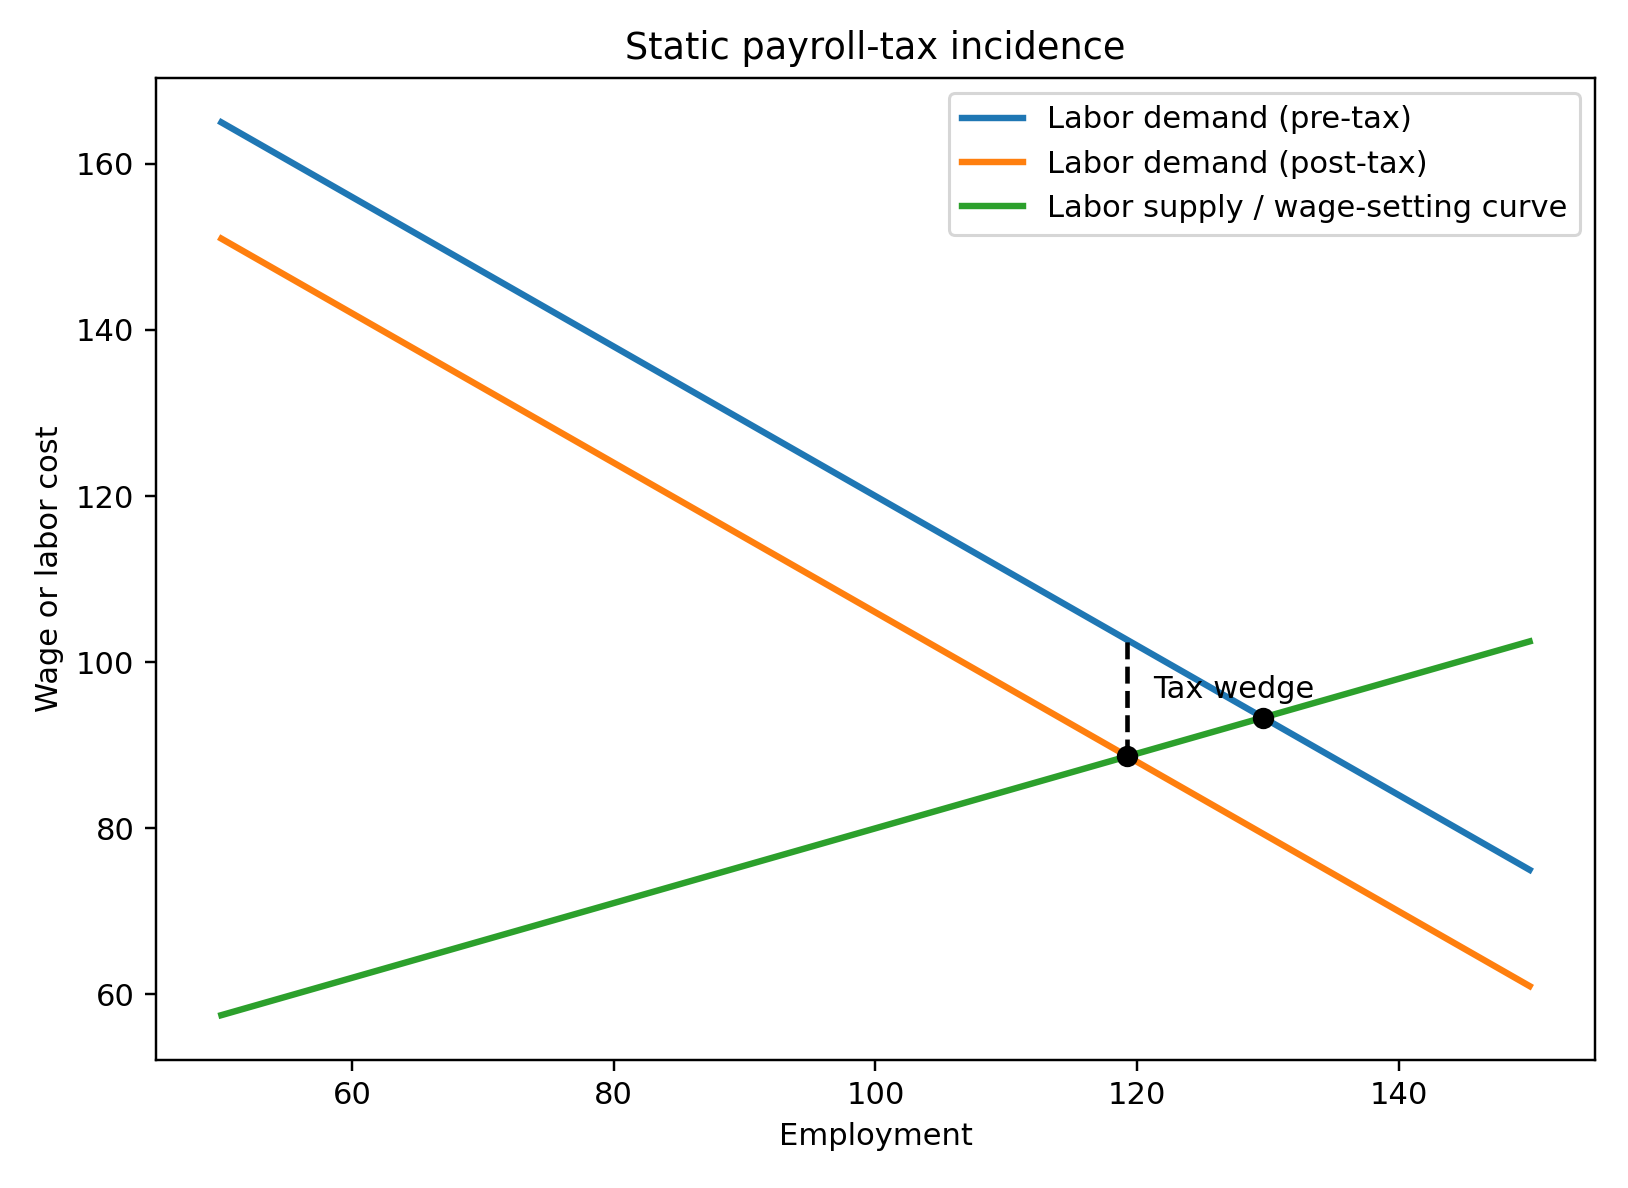
\includegraphics[width=0.82\linewidth]{01-payroll-tax-incidence.png}
\end{center}
\end{frame}

\begin{frame}{Empirical design map}
\small
\begin{tabular}{p{0.24\linewidth} p{0.21\linewidth} p{0.22\linewidth} p{0.23\linewidth}}
\toprule
Design & Variation & Margin & Core object \\
\midrule
Payroll-tax reform & Labor cost & Employment, wages & Total demand and incidence \\
City-industry shock & Local demand & Employment, wages & Demand with spillovers \\
Product-market cost shock & Marginal cost & Prices, employment & Product-demand link \\
Rent sharing & Firm rents & Wages, firm-worker outcomes & Boundary with wage-setting \\
\bottomrule
\end{tabular}
\end{frame}

\begin{frame}{Bridge to Week 2}
\begin{itemize}
    \item Week 1 tells us the firm's target after a shock.
    \item Week 2 asks why hiring and firing frictions slow movement toward that target.
    \item Dynamic adjustment costs turn a comparative-static destination into an employment path.
\end{itemize}
\end{frame}

\begin{frame}{Takeaways}
\begin{itemize}
    \item Labor demand is derived from technology, costs, and product demand.
    \item Conditional demand is a substitution object; total demand adds scale.
    \item Hicks--Marshall logic disciplines policy incidence and empirical interpretation.
    \item Week 2 starts once we admit firms cannot jump to the new optimum costlessly.
\end{itemize}
\end{frame}

\end{document}
